\section{Optical Excitations}

The parent compound displays valley selectivity.
One circular polarization couples to one valley
and the opposite to the other.
Here, we investigate the extent to which this property
is inherited by the superconducting phase.
Note that the orbitals involved have the same parity,
this one does not expect any dipolar coupling.
The optical excitations arise from the Berry curvature,
which acts as an effective angular momentum.
The electromagnetic potential $\vc{A}$,
with polarization vector $\vc{ϵ}$,
is introduced using minimal coupling,
\begin{equation}
  H_{τ σ}^{ν ν'} \ofK
  → H_{τ σ}^{ν ν'} \of{\vK + e \vc{A}},
\end{equation}
where, in the dipole approximation,
$\vc{A} = 2 \re{\vc{ϵ} A_0 e^{- i ω t}}$.
This yields a perturbed Hamiltonian
$H → H + H^A$, where
$H^A = H' e^{- i ω t} + H'^† e^{i ω t}$,
\begin{multline}
  H'
  = \sumK ∑_{τ, σ}
    H'_τ
    {a^v_{τ σ}}^† \ofK
    a^c_{τ σ} \ofK \\
  - \sumK ∑_{τ, σ}
    H'_{-τ}
    {a^c_{τ σ}}^† \ofK
    a^v_{τ σ} \ofK,
\end{multline}
and
\begin{equation}
  H'_τ
  = a t e A_0
    \left( τ \vc{\hat{x}} + i \vc{\hat{y}} \right)
    · \vc{ϵ}.
\end{equation}
The transition rate is proportional to the modulus-squared
of the optical matrix elements,
$\vc{P}_{τ σ}^{n n'} \ofK$,
defined by
\begin{multline}
  H^A
  = ∑_{\substack{\vK, τ, σ \\ n, n'}}
    \frac{e A_0}{m_0}
    \vc{ϵ} · \vc{P}_{τ σ}^{n n'} \ofK
    {c_{τ σ}^n}^† \ofK
    c_{τ σ}^{n'} \ofK.
\end{multline}

For circularly polarized light, in the absence of superconductivity,
$\vc{ϵ}_± = \left( \vc{\hat{x}} ± i \vc{\hat{y}} \right) / \sqrt{2}$,
\begin{equation}
  \label{eq:optical}
  \vc{ϵ}_± · \vc{P}_{τ σ}^{+ -} \of{\vK}
  = ∓ τ \sqrt{2} a t m_0
    e^{± i ϕ}
    \sin^2 {\frac{\fnTheta{∓ τ}}{2}}.
\end{equation}
Since $\fnTheta{-} - \fnTheta{+} = τ π$,
switching either valley or polarization transforms
$\sin → \cos$ in \cref{eq:optical},
leading to the valley selectivity in optical excitation.
For excitations above the BCS state,
the transition rate is given by \cref{eq:optical}
multiplied by a coherence factor $\sin^2 {β_{\vK}}$.
Thus, the superconducting phase exhibits
the same strong optical-valley coupling
for circularly polarized light.
This is shown in \cref{fig:optical.transitions}.
\begin{figure}
  \caption{%
    Optical transition rate matrix elements
    $\left| P_± \right|
    = \left(c / ℏ \right) \left| \vc{ϵ_±} · P_+^{+ -} \sin {β} \right|$
    for \ce{MoSe2}, \ce{WS2}, and \ce{WSe2}.
  }\label{fig:optical.transitions}
  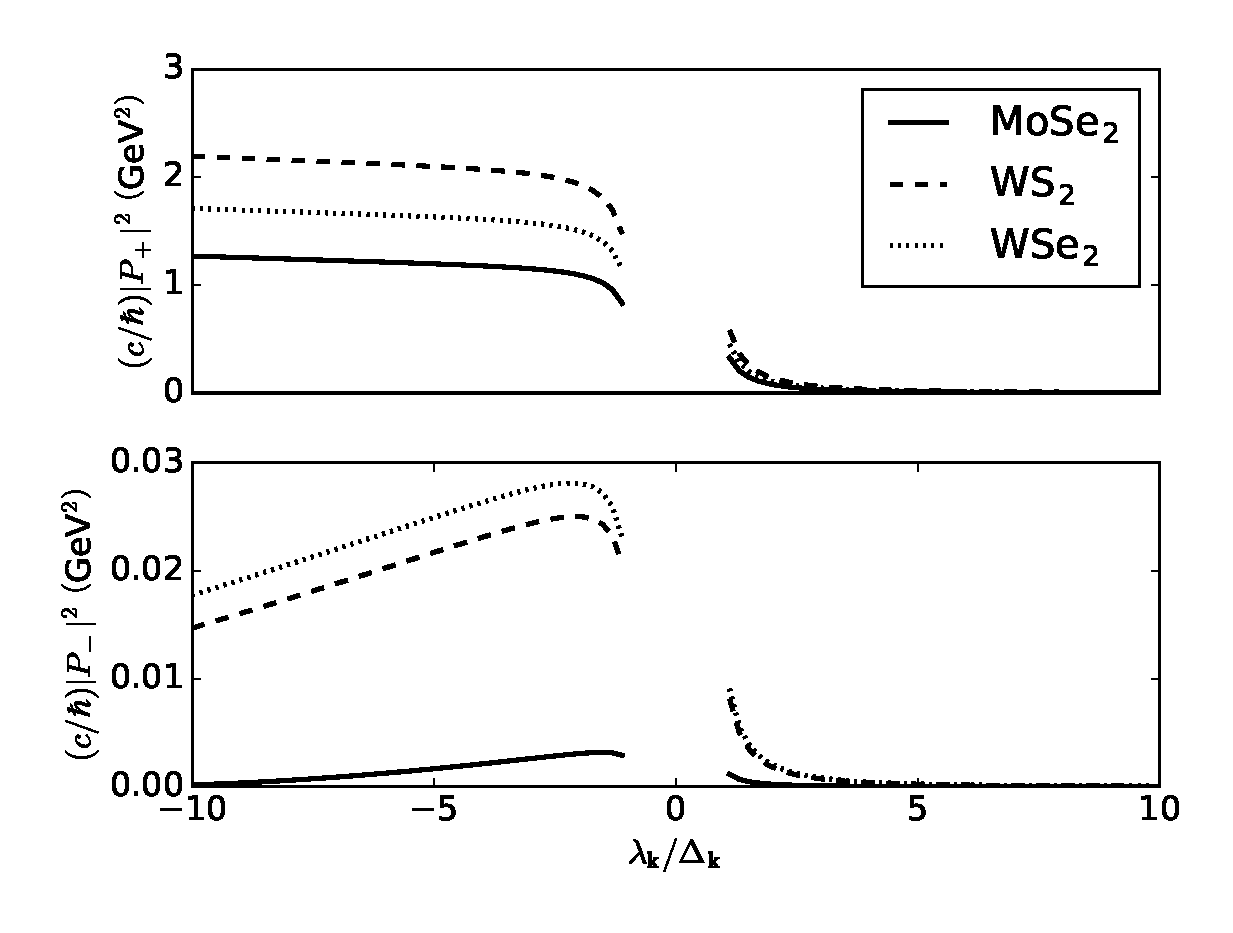
\includegraphics[width=\columnwidth]{figures/optical-transitions}
\end{figure}

For a given valley, a given polarity of light couples more strongly
than the other, as is evident comparing $\abs{P_+}$ to $\abs{P_-}$.
The suppression of the matrix elements above the chemical potential
reflects the fact that the BCS states include the Fermi distribution.
As such, the matrix element is still finite,
but is multiplied by an occupation probability which is vanishing.
The key new feature is the suppression of the valley contrast
as one approaches the chemical potential.
Nevertheless, for energies where the cooper pair
is broken into quasiparticles well above the gap,
valley selective phenomena of the parent compound
is inherited by the superconducting state.
